\documentclass{article}

\usepackage[margin=2.5cm,left=2cm,includefoot]{geometry}
\usepackage{graphicx}
\usepackage{float}
\usepackage[space]{grffile}
\usepackage{hyperref}
\usepackage[export]{adjustbox}
\usepackage{multicol}
\usepackage{caption}
\usepackage{hyperref}
\usepackage{listings}
\usepackage{vhistory}
\newcommand{\nexists}{\not\exists}
\newcommand\tab[1][0.5cm]{\hspace*{#1}}

\usepackage{tabulary}
\newcolumntype{K}[1]{>{\centering\arraybackslash}p{#1}}


\usepackage{titlesec}

\setcounter{secnumdepth}{4}

\titleformat{\paragraph}
{\normalfont\normalsize\bfseries}{\theparagraph}{1em}{}
\titlespacing*{\paragraph}
{0pt}{3.25ex plus 1ex minus .2ex}{1.5ex plus .2ex}

% Header and footer
\usepackage{fancyhdr}
\pagestyle{fancy}

\rhead{COS301}
\lhead{Functional Specification}
\fancyfoot[R]{Page \thepage}

\renewcommand{\headrulewidth}{2pt}
\renewcommand{\footrulewidth}{1pt}

\begin{document}

	\begin{titlepage}
		\begin{center}
			
\includegraphics[width=10cm]{images/UP.jpg}  \\
			[0.5cm]
			\huge{
			Functional Specification\\
			}

			\line(1,0){300}\\
			[0.2cm]
			\LARGE{Project: Insurance profiling from social media\\
			Client: RetroRabbit} \\
			\line(1,0){300}\\
			\LARGE{Team: Valknut Solutions}\\
			[1.0cm]
			\large
			{
			\begin{itemize}
				\item 13054903 - Charl Jansen van Vuuren
				\item 13044924 - Kevin Heritage
				\item 13176545 - Quinton Weenink\\
			\end{itemize}
			}
			\textsc{\large}\\
		[3.0cm]
		\textsc{\large  Department of Computer Science}\\
		[0.5cm]
		\textsc{\large \today}\\
		\end{center}

		%\begin{figure}[H]}
		%\centering
		%\includegraphics[{imagename}
		%\end{figure}\

	\end{titlepage}
	\cleardoublepage
	\tableofcontents
	\cleardoublepage
	% Start of the revision history table
	\begin{versionhistory}
  		\vhEntry{1.0}{27.05.2016}{CJvV,KH,QW}{Original Architectural document without Functional requirements}
  		\vhEntry{1.1}{27.07.2016}{CJvV,KH,QW}{Added Functional requirements and separated Architectural requirements}
		\vhEntry{1.2}{27.07.2016}{CJvV,KH,QW}{Added better scoping requirements}
	\end{versionhistory}

\section{Functional requirements and application design}
	\subsection{Scope}
		\begin{figure}[H]
		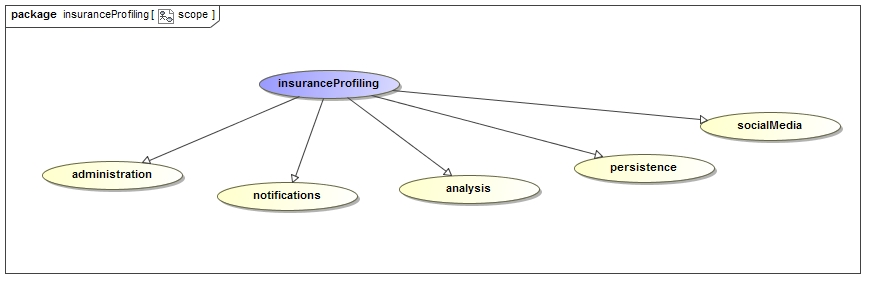
\includegraphics[width=\textwidth]{images/uc__insuranceProfiling__scope.jpg}  \\
		\caption{Scope : Insurance Profiling}
		\end{figure}
	\subsection{Social Media subsystem}
		\subsubsection{Use cases}

		\begin{figure}[H]
		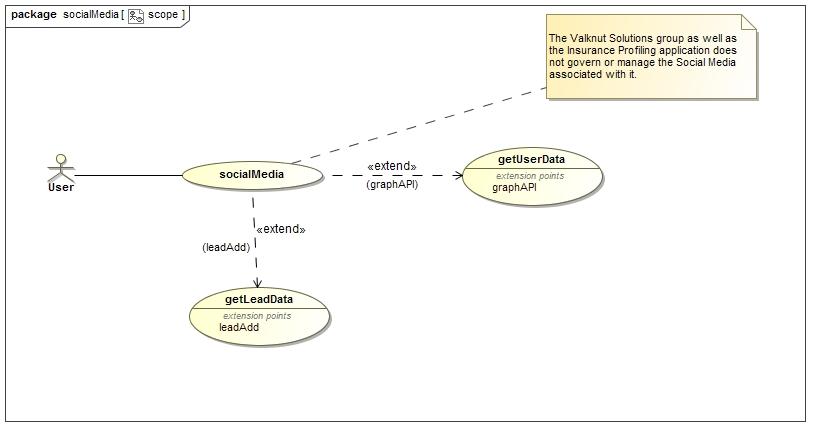
\includegraphics[width=\textwidth]{images/uc__socialMedia__scope.jpg}  \\
		\caption{Use Case Diagram : Social Media}
		\end{figure}

		\begin{flushleft}
			\textbf{Critical}
				\begin{itemize}
	  				\item validateUser
	  				\item createUser
	  				\item getUser
				\end{itemize}
			\textbf{Important}
				\begin{itemize}
	  				\item validateUser
				\end{itemize}

			\textbf{Nice-To-Have}
				\begin{itemize}
	  				\item getAnalyst
	  				\item analiseUser
				\end{itemize}
		\end{flushleft}

		\subsubsection{Services Contracts}

		\begin{figure}[H]
		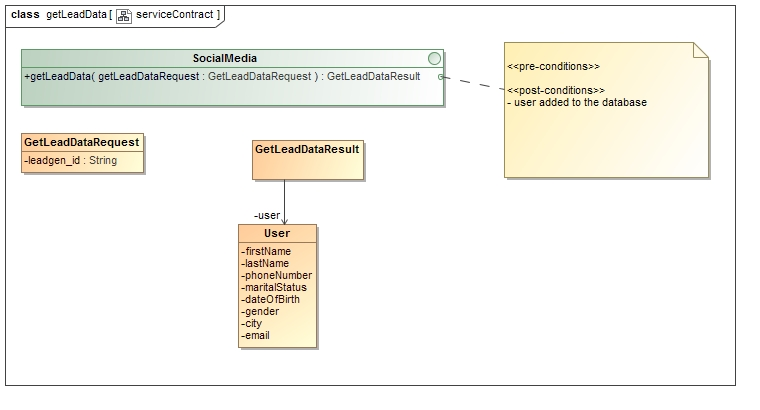
\includegraphics[width=\textwidth]{images/class__getLeadData__serviceContract.jpg}  \\
		\caption{Service Contract : addLeadData}
		\end{figure}

		\subsubsection{Required Functionality}

		\begin{figure}[H]
		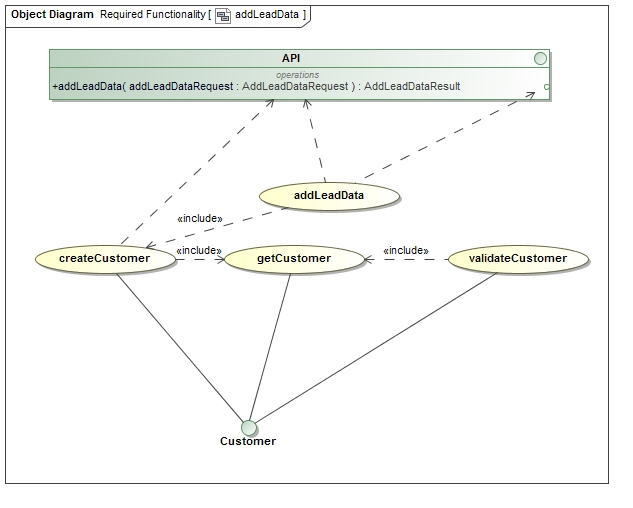
\includegraphics[width=\textwidth]{images/obj__Required_Functionality__addLeadData.jpg}  \\
		\caption{Required Functionality : addLeadData}
		\end{figure}

		\subsubsection{Process specifications}

		\begin{figure}[H]
		%
\includegraphics[width=\textwidth]{images/Incomplete.png}  \\
		\caption{Process specification : Publications}
		\end{figure}

	\subsection{Analysis subsystem}
		\subsubsection{Use cases}

		\begin{figure}[H]
		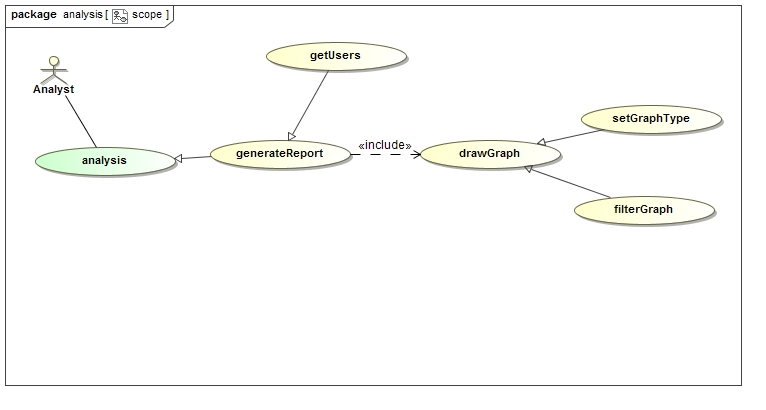
\includegraphics[width=\textwidth]{images/uc__analysis__scope.jpg}  \\
		\caption{Use Case Diagram : Analysis}
		\end{figure}

		\begin{flushleft}
			\textbf{Critical}
				\begin{itemize}
					\item validateUser
					\item createUser
					\item getUser
				\end{itemize}
			\textbf{Important}
				\begin{itemize}
					\item validateUser
				\end{itemize}

			\textbf{Nice-To-Have}
				\begin{itemize}
					\item getAnalyst
					\item analiseUser
				\end{itemize}
		\end{flushleft}

		\subsubsection{Services Contracts}

		\begin{figure}[H]
		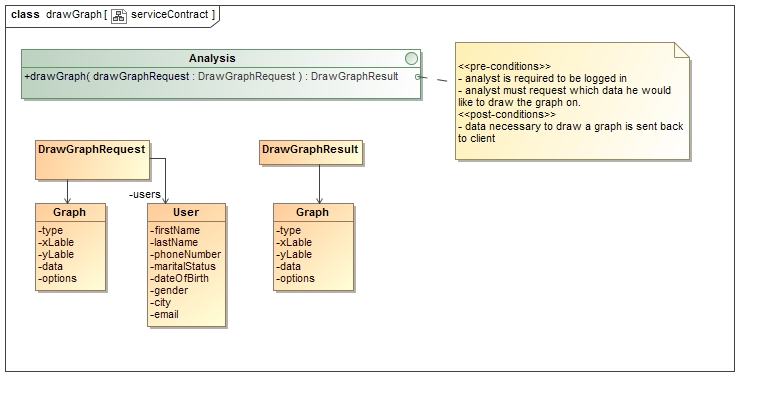
\includegraphics[width=\textwidth]{images/class__drawGraph__serviceContract.jpg}  \\
		\caption{Service Contract : drawGraph}
		\end{figure}

		\subsubsection{Required Functionality}

		\begin{figure}[H]
		%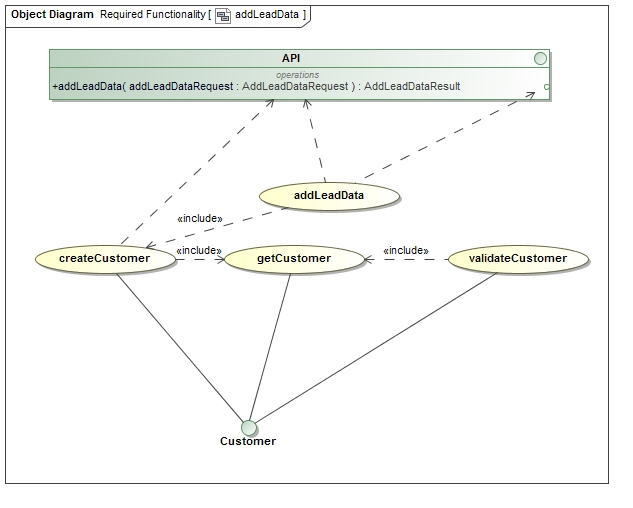
\includegraphics[width=\textwidth]{images/obj__Required_Functionality__addLeadData.jpg}  \\
		\caption{Required Functionality : drawGraph}
		\end{figure}

		\subsubsection{Process specifications}

		\begin{figure}[H]
		%
\includegraphics[width=\textwidth]{images/Incomplete.png}  \\
		\caption{Process specification : drawGraph}
		\end{figure}

	\subsection{Administration subsystem}
		\subsubsection{Use cases}

		\begin{figure}[H]
		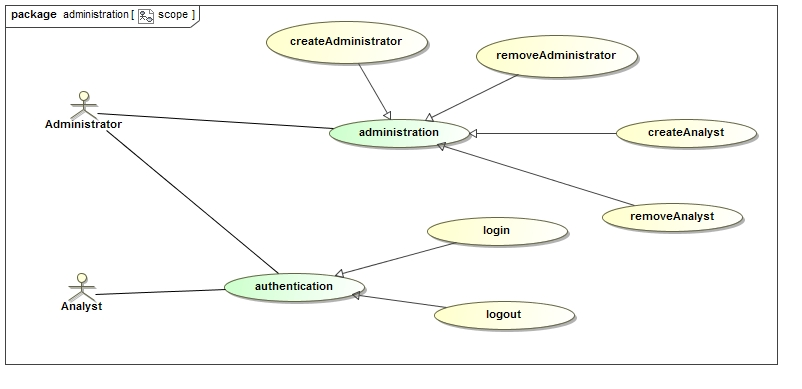
\includegraphics[width=\textwidth]{images/uc__administration__scope.jpg}  \\
		\caption{Use Case Diagram : Administration}
		\end{figure}

		\begin{flushleft}
			\textbf{Critical}
				\begin{itemize}
					\item validateUser
					\item createUser
					\item getUser
				\end{itemize}
			\textbf{Important}
				\begin{itemize}
					\item validateUser
				\end{itemize}

			\textbf{Nice-To-Have}
				\begin{itemize}
					\item getAnalyst
					\item analiseUser
				\end{itemize}
		\end{flushleft}

		\subsubsection{Services Contracts}

		\begin{figure}[H]
		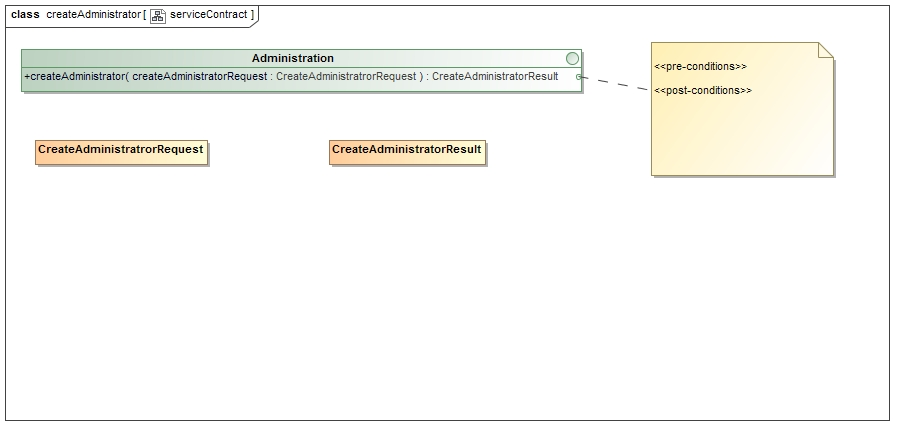
\includegraphics[width=\textwidth]{images/class__createAdministrator__serviceContract.jpg}  \\
		\caption{Service Contract : createAdministrator}
		\end{figure}

		\begin{figure}[H]
		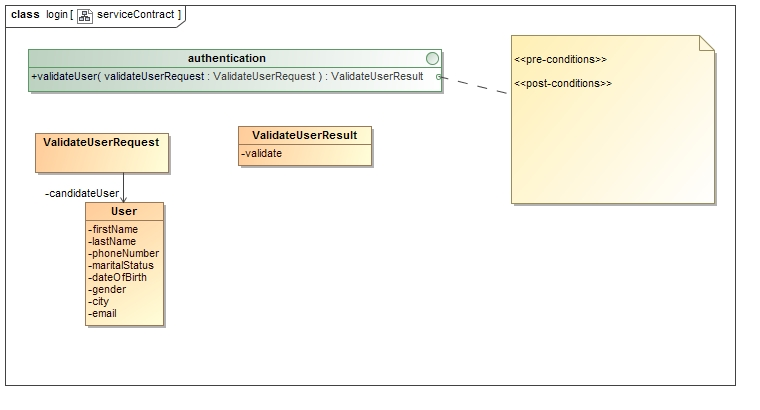
\includegraphics[width=\textwidth]{images/class__login__serviceContract.jpg}  \\
		\caption{Service Contract : login}
		\end{figure}

		\subsubsection{Required Functionality}

		\begin{figure}[H]
		%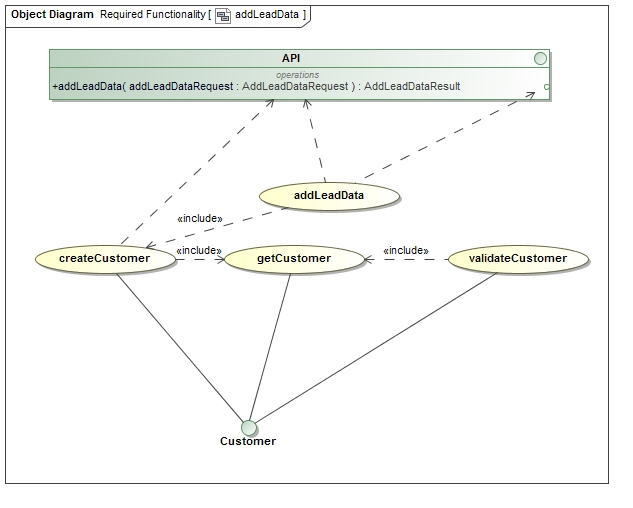
\includegraphics[width=\textwidth]{images/obj__Required_Functionality__addLeadData.jpg}  \\
		\caption{Required Functionality : createAdministrator}
		\end{figure}

		\subsubsection{Process specifications}

		\begin{figure}[H]
		%
\includegraphics[width=\textwidth]{images/Incomplete.png}  \\
		\caption{Process specification : createAdministrator}
		\end{figure}

	\subsection{Persistence subsystem}
		\subsubsection{Use cases}

		\begin{figure}[H]
		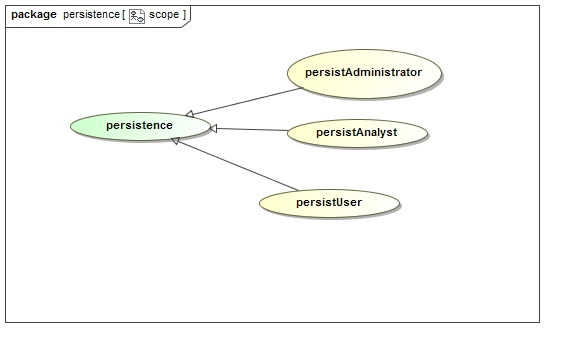
\includegraphics[width=\textwidth]{images/uc__persistence__scope.jpg}  \\
		\caption{Use Case Diagram : Persistence}
		\end{figure}

		\begin{flushleft}
			\textbf{Critical}
				\begin{itemize}
					\item validateUser
					\item createUser
					\item getUser
				\end{itemize}
			\textbf{Important}
				\begin{itemize}
					\item validateUser
				\end{itemize}

			\textbf{Nice-To-Have}
				\begin{itemize}
					\item getAnalyst
					\item analiseUser
				\end{itemize}
		\end{flushleft}

		\subsubsection{Services Contracts}

		\begin{figure}[H]
		%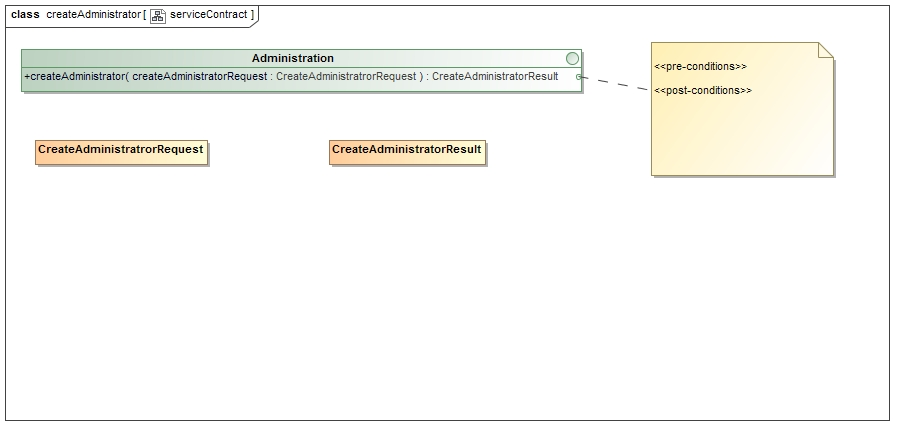
\includegraphics[width=\textwidth]{images/class__createAdministrator__serviceContract.jpg}  \\
		\caption{Service Contract : persistUser}
		\end{figure}

		\subsubsection{Required Functionality}

		\begin{figure}[H]
		%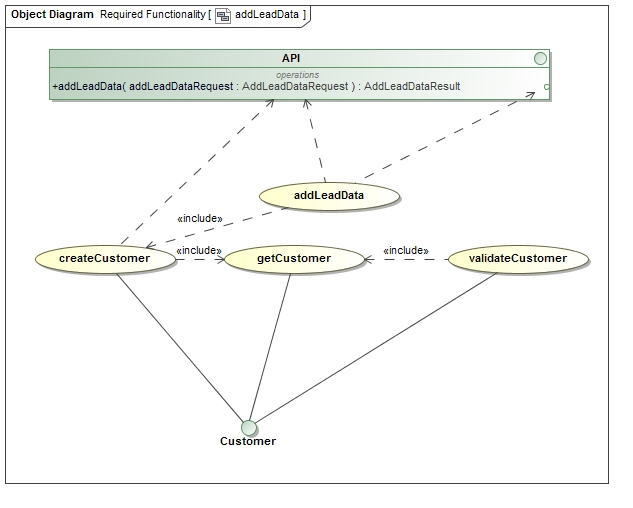
\includegraphics[width=\textwidth]{images/obj__Required_Functionality__addLeadData.jpg}  \\
		\caption{Required Functionality : persistUser}
		\end{figure}

		\subsubsection{Process specifications}

		\begin{figure}[H]
		%
\includegraphics[width=\textwidth]{images/Incomplete.png}  \\
		\caption{Process specification : persistUser}
		\end{figure}

	\subsection{Notifications subsystem}
		\subsubsection{Use cases}

		\begin{figure}[H]
		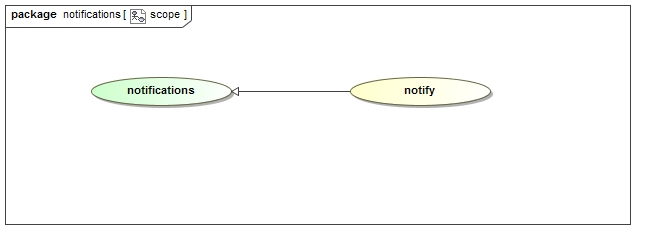
\includegraphics[width=\textwidth]{images/uc__notifications__scope.jpg}  \\
		\caption{Use Case Diagram : Notifications}
		\end{figure}

		\begin{flushleft}
			\textbf{Critical}
				\begin{itemize}
					\item validateUser
					\item createUser
					\item getUser
				\end{itemize}
			\textbf{Important}
				\begin{itemize}
					\item validateUser
				\end{itemize}

			\textbf{Nice-To-Have}
				\begin{itemize}
					\item getAnalyst
					\item analiseUser
				\end{itemize}
		\end{flushleft}

		\subsubsection{Services Contracts}

		\begin{figure}[H]
		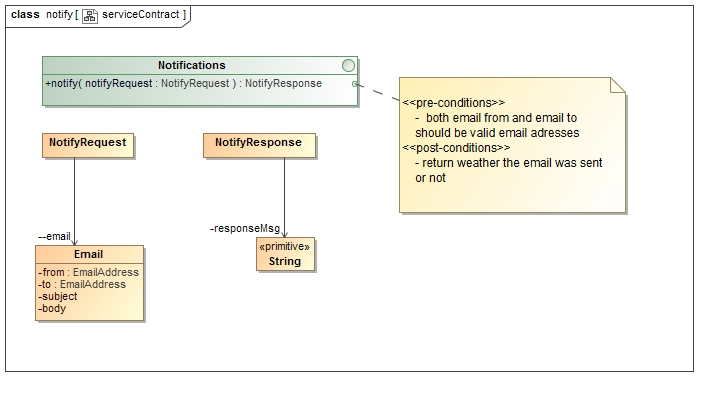
\includegraphics[width=\textwidth]{images/class__notify__serviceContract.jpg}  \\
		\caption{Service Contract : notify}
		\end{figure}

		\subsubsection{Required Functionality}

		\begin{figure}[H]
		%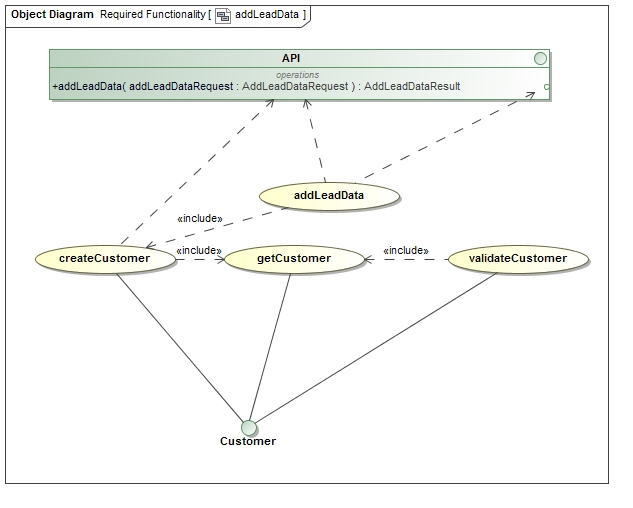
\includegraphics[width=\textwidth]{images/obj__Required_Functionality__addLeadData.jpg}  \\
		\caption{Required Functionality : notify}
		\end{figure}

		\subsubsection{Process specifications}

		\begin{figure}[H]
		%
\includegraphics[width=\textwidth]{images/Incomplete.png}  \\
		\caption{Process specification : notify}
		\end{figure}


\subsection{Domain model}

\begin{figure}[H]
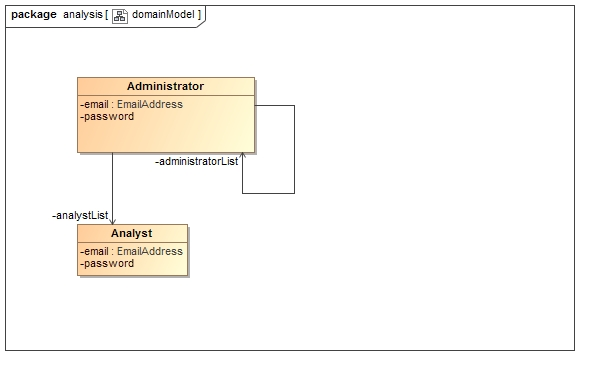
\includegraphics[width=\textwidth]{images/class__analysis__domainModel.jpg}  \\
\caption{Domain Model : Analysis}
\end{figure}

\begin{figure}[H]
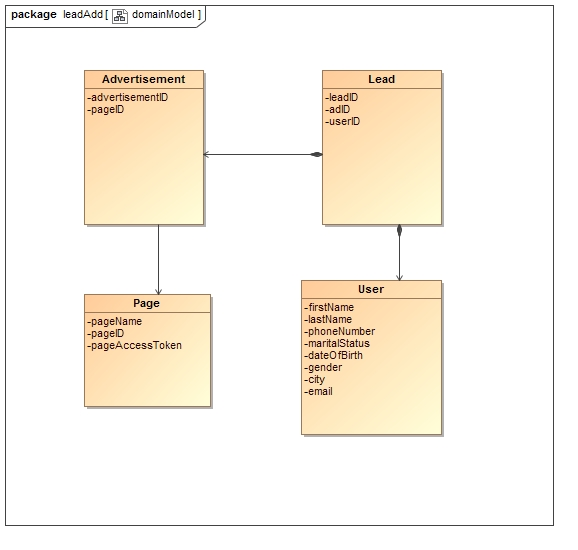
\includegraphics[width=\textwidth]{images/class__leadAdd__domainModel.jpg}  \\
\caption{Domain Model : Social Media}
\end{figure}

\subsection{Open Issues}






\end{document}
